% This file was converted to LaTeX by Writer2LaTeX ver. 1.0.2
% see http://writer2latex.sourceforge.net for more info
\documentclass[a4paper]{article}
\usepackage[ascii]{inputenc}
\usepackage[T1]{fontenc}
\usepackage[spanish,dutch,english]{babel}
\usepackage{amsmath}
\usepackage{amssymb,amsfonts,textcomp}
\usepackage{color}
\usepackage{array}
\usepackage{supertabular}
\usepackage{hhline}
\usepackage{hyperref}
\hypersetup{pdftex, colorlinks=true, linkcolor=blue, citecolor=blue, filecolor=blue, urlcolor=blue, pdftitle=, pdfauthor=Ruben Perez Pascual, pdfsubject=, pdfkeywords=}
\usepackage[pdftex]{graphicx}
% Outline numbering
\setcounter{secnumdepth}{3}
\renewcommand\thesection{\arabic{section}}
\renewcommand\thesubsection{\arabic{section}.\arabic{subsection}}
\renewcommand\thesubsubsection{\arabic{section}.\arabic{subsection}.\arabic{subsubsection}}
\makeatletter
\newcommand\arraybslash{\let\\\@arraycr}
\makeatother
% List styles
\newcounter{saveenum}
\newcommand\liststyleLFOiii{%
\renewcommand\labelitemi{[F0B7?]}
\renewcommand\labelitemii{o}
\renewcommand\labelitemiii{[F0A7?]}
\renewcommand\labelitemiv{[F0B7?]}
}
\newcommand\liststyleLFOvi{%
\renewcommand\theenumi{\roman{enumi}}
\renewcommand\theenumii{\alph{enumii}}
\renewcommand\theenumiii{\roman{enumiii}}
\renewcommand\theenumiv{\arabic{enumiv}}
\renewcommand\labelenumi{\theenumi)}
\renewcommand\labelenumii{\theenumii.}
\renewcommand\labelenumiii{\theenumiii.}
\renewcommand\labelenumiv{\theenumiv.}
}
\newcommand\liststyleLFOv{%
\renewcommand\theenumi{\arabic{enumi}}
\renewcommand\labelenumi{\theenumi.}
\renewcommand\labelitemi{o}
\renewcommand\labelitemii{[F0A7?]}
\renewcommand\labelitemiii{[F0B7?]}
}
\newcommand\liststyleLFOiv{%
\renewcommand\labelitemi{[F0B7?]}
\renewcommand\labelitemii{o}
\renewcommand\labelitemiii{[F0A7?]}
\renewcommand\labelitemiv{[F0B7?]}
}
\newcommand\liststyleLFOvii{%
\renewcommand\theenumi{\arabic{enumi}}
\renewcommand\theenumii{\roman{enumii}}
\renewcommand\theenumiii{\arabic{enumiii}}
\renewcommand\labelenumi{\theenumi.}
\renewcommand\labelitemi{[F0D8?]}
\renewcommand\labelenumii{\theenumii.}
\renewcommand\labelenumiii{\theenumiii.}
}
\newcommand\liststyleLFOviii{%
\renewcommand\theenumi{\arabic{enumi}}
\renewcommand\theenumii{\roman{enumii}}
\renewcommand\theenumiii{\arabic{enumiii}}
\renewcommand\labelenumi{\theenumi.}
\renewcommand\labelitemi{o}
\renewcommand\labelenumii{\theenumii.}
\renewcommand\labelenumiii{\theenumiii.}
}
\newcommand\liststyleLFOix{%
\renewcommand\theenumi{\arabic{enumi}}
\renewcommand\theenumii{\roman{enumii}}
\renewcommand\theenumiii{\arabic{enumiii}}
\renewcommand\labelenumi{\theenumi.}
\renewcommand\labelitemi{o}
\renewcommand\labelenumii{\theenumii.}
\renewcommand\labelenumiii{\theenumiii.}
}
\newcommand\liststyleLFOx{%
\renewcommand\theenumi{\arabic{enumi}}
\renewcommand\theenumii{\roman{enumii}}
\renewcommand\theenumiii{\arabic{enumiii}}
\renewcommand\labelenumi{\theenumi.}
\renewcommand\labelitemi{o}
\renewcommand\labelenumii{\theenumii.}
\renewcommand\labelenumiii{\theenumiii.}
}
\newcommand\liststyleLFOxi{%
\renewcommand\theenumi{\arabic{enumi}}
\renewcommand\theenumii{\roman{enumii}}
\renewcommand\theenumiii{\arabic{enumiii}}
\renewcommand\labelenumi{\theenumi.}
\renewcommand\labelitemi{o}
\renewcommand\labelenumii{\theenumii.}
\renewcommand\labelenumiii{\theenumiii.}
}
\newcommand\liststyleLFOxii{%
\renewcommand\theenumi{\arabic{enumi}}
\renewcommand\theenumii{\roman{enumii}}
\renewcommand\theenumiii{\arabic{enumiii}}
\renewcommand\labelenumi{\theenumi.}
\renewcommand\labelitemi{o}
\renewcommand\labelenumii{\theenumii.}
\renewcommand\labelenumiii{\theenumiii.}
}
\newcommand\liststyleLFOxiii{%
\renewcommand\theenumi{\arabic{enumi}}
\renewcommand\theenumii{\roman{enumii}}
\renewcommand\theenumiii{\arabic{enumiii}}
\renewcommand\labelenumi{\theenumi.}
\renewcommand\labelitemi{o}
\renewcommand\labelenumii{\theenumii.}
\renewcommand\labelenumiii{\theenumiii.}
}
% Page layout (geometry)
\setlength\voffset{-1in}
\setlength\hoffset{-1in}
\setlength\topmargin{0.4923in}
\setlength\oddsidemargin{0.9847in}
\setlength\textheight{9.7238in}
\setlength\textwidth{6.2985992in}
\setlength\footskip{0.4923in}
\setlength\headheight{0.4923in}
\setlength\headsep{0cm}
% Footnote rule
\setlength{\skip\footins}{1.1777999mm}
\renewcommand\footnoterule{\vspace*{-0.007in}\setlength\leftskip{0pt}\setlength\rightskip{0pt plus 1fil}\noindent\textcolor{black}{\rule{0.33\columnwidth}{0.007in}}\vspace*{1mm}}
% Pages styles
\makeatletter
\newcommand\ps@MP{
  \renewcommand\@oddhead{FP7-ICT-318389/DEIMOS/REPORT/CO/GEO-Cloud-DMS-TEC-TEC12-E}
  \renewcommand\@evenhead{\@oddhead}
  \renewcommand\@oddfoot{}
  \renewcommand\@evenfoot{\@oddfoot}
  \renewcommand\thepage{\arabic{page}}
}
\makeatother
\pagestyle{MP}
\setlength\tabcolsep{1mm}
\renewcommand\arraystretch{1.3}
\title{}
\author{Ruben Perez Pascual}
\date{2014-07-04T11:20:00Z}
\begin{document}
\begin{flushleft}
\tablehead{}
\begin{supertabular}{llll}
\multicolumn{1}{c}{

\includegraphics[width=1.43472in,height=1.30417in]{ple-img1.png} } &
\multicolumn{1}{c}{~
} & \multicolumn{1}{c}{~
} & \multicolumn{1}{c}{

\includegraphics[width=1.35625in,height=0.92153in]{ple-img2.jpg} }\\
\end{supertabular}
\end{flushleft}

\bigskip


\bigskip

\begin{flushleft}
\tablehead{}
\begin{supertabular}{|m{1.98856in}|m{4.25246in}|}
\hline
Project Acronym &
\bfseries Fed4FIRE\\\hline
Project Title &
\bfseries Federation for FIRE\\\hline
Instrument &
\bfseries Large scale integrating project (IP)\\\hline
Call identifier &
\bfseries FP7-ICT-2011-8\\\hline
Project number &
\bfseries 318389\\\hline
Project website &
\bfseries www.fed4fire.eu\\\hline
Experiment &
\bfseries GEO-Cloud\\\hline
\end{supertabular}
\end{flushleft}

\bigskip


\bigskip

{\centering\bfseries
Implementation of PL Experiment
\par}


\bigskip

\begin{flushleft}
\tablehead{}
\begin{supertabular}{|m{1.9649599in}|m{4.27466in}|}
\hline
Work\ package &
WP10\\\hline
Task &
T10.1.2\ GEO-Cloud Experiment\\\hline
Due date &
09/05/2014\\\hline
Submission date &
09/05/2014\\\hline
Report Lead &
F\'elix Pedrera\ (DEIMOS)\\\hline
Version &
1.0\\\hline
Authors &
\foreignlanguage{spanish}{Manuel Jos\'e Latorre, F\'elix
Pedrera,\ }\foreignlanguage{spanish}{\ }\foreignlanguage{dutch}{Miguel
Lizondo, C\'esar Gonz\'alez, Esteban
Bueno,\ }\foreignlanguage{spanish}{Rub\'en
P\'erez\ }\foreignlanguage{spanish}{(DEIMOS)}\foreignlanguage{dutch}{\ }\\\hline
Reviewers &
Jonathan Becedas\ (DEIMOS)\\\hline
\end{supertabular}
\end{flushleft}

\bigskip


\bigskip

\begin{flushleft}
\tablehead{}
\begin{supertabular}{|m{1.9649599in}|m{4.27466in}|}
\hline
\bfseries Document ID &
\selectlanguage{spanish}\bfseries GEO-Cloud-DMS-TEC-TEC12-E\\\hline
Abstract &
This document provides\ technical information about\ the\ implementation
of the experiment in PlanetLab\\\hline
Keywords &
Report\\\hline
\end{supertabular}
\end{flushleft}

\bigskip


\bigskip

\begin{flushleft}
\tablehead{}
\begin{supertabular}{m{1.9649599in}|m{0.31495985in}|m{3.36706in}|m{0.43505988in}|}
\hline
\multicolumn{1}{|m{1.9649599in}|}{Nature of the\ document} &
R &
Report &
X\\\hline
 &
P &
Prototype &
~
\\\hhline{~---}
 &
D &
Demonstrator &
~
\\\hhline{~---}
 &
O &
Other &
~
\\\hline
\multicolumn{1}{|m{1.9649599in}|}{Dissemination level} &
PU &
Public &
~
\\\hline
 &
PP &
Restricted to other programme participants (including the Commission) &
~
\\\hhline{~---}
 &
RE &
Restricted to a group specified by the consortium (including the
Commision) &
~
\\\hhline{~---}
 &
CO &
Confidential, only for members of the consortium (including the
Commission) &
X\\\hhline{~---}
\end{supertabular}
\end{flushleft}

\bigskip

\clearpage
\textrm{\textbf{Disclaimer}}


\bigskip

\textit{The information, documentation and figures available in this
deliverable, is written by the Fed4FIRE\ }(Federation for
FIRE)\ \textit{{}-- project consortium under EC co-financing contract
FP7-ICT-}\textit{318389}\textit{\ and does not necessarily reflect the
views of the European Commission}\textit{. The European
C}\textit{ommission is not liable for any use that may be made of the
information contained herein.}

\clearpage
\textrm{\textbf{Executive S}}\textrm{\textbf{ummary}}

In\ this\ document the implementation of the experiment in PlanetLab\ is
described. This experiment has as objective the measurements
of\ the\ network impairments to model a real network. These impairments
will be implemented in the network that communicates the simulators
implemed in Virtual Wall \ with the BonFIRE cloud.\ 

\clearpage
\textrm{\textbf{A}}\textrm{\textbf{cronyms and
A}}\textrm{\textbf{bbreviations}}


\bigskip

\begin{flushleft}
\tablehead{}
\begin{supertabular}{|m{0.8823598in}|m{5.35596in}|}
\hline
PL &
PlanetLab\\\hline
VM &
Virtual Machine\\\hline
VW &
Virtual Wall\\\hline
\end{supertabular}
\end{flushleft}
\clearpage
\textrm{\textbf{Table of C}}\textrm{\textbf{ontents}}


\bigskip

\setcounter{tocdepth}{3}
\tableofcontents

\bigskip

\section[Introduction]{Introduction}
\hypertarget{Toc387315382}{}The GEO-Cloud experiment is separated into
two experiments: i) an experiment that represents a complete Earth
Observation system, including the space system communicated with a
cloud base data center for the ingestion, processing, storage and
distribution of satellite imagery through high added value web services
(Virtual Wall and BonFIRE are the testbeds used); ii) an experiment to
measure and model the network that links the space system with the
cloud\ as realistically as possible.\ The results of this experiment
carried out in PlanetLab are used to link the simulators implemented in
Virtual Wall with the cloud in BonFIRE to simulate a real network with
realistic characteristics.


\bigskip

This document is devoted to explain the implementation of the experiment
in PlanetLab.\ \ First, the motivation for the use of PlanetLab is
explained together with the design of the real system. Then, the
platform and tools used are described with their roles in the
experiment. In addition, the network and experiment design are broadly
discussed. The execution of the experiment is also presented. Finally,
conclusions of this implementation are included.


\bigskip


\bigskip


\bigskip

\section{Definitions}

\bigskip

\textit{E}\textit{ffective bandwidth (Mbps)}\ is the actual bandwidth at
which the data can be transmitted on a link. The nominal bandwidth
cannot be reached due to network congestion, the distance between
nodes, delays, etc. Effective bandwidth is higher when nodes are
closer, the congestion is scarce and the delays in the transmission are
not long.

\textit{Bandwidth\ }\textit{of the
network}\textit{(Mbps)}\textit{,}\ which is\ the
nominal\ {\textquotedblleft}width{\textquotedblright}\ of the channel
used, if the bandwidth increases, more data can simultaneously be sent,
reducing the necessary time to transfer a packet of data. It is usually
confused with the signal velocity, which affects the time the data
takes to travel to the receiver (latency) but bandwidth cannot reduce
this time.

\textit{Loss rate\ }is the fraction of data lost in the communication
with respect to all the data sent. It is a value between 0 and 1.\ It
can also be provided in percentage.

\textit{Latency (ms)}\ is the time it takes a signal to travel from its
source, trough the communication channel, until it reaches the
receiver. It is related with the distance between the nodes, the
network congestion and\ the propagation velocity (a fraction of the
light speed) among other parameters.\ 


\bigskip

\section[Platforms and Tools Description]{Platforms and Tools
Description}
\hypertarget{Toc387315383}{}The experiment presented in this\ report\ is
completely carried out in PlanetLab, although the results\ obtained
will be\ used to implement a realistic model of the networks in the
communications between the simulators and the cloud system of the
GEOCloud experiment implemented in Virtual Wall and BonFIRE
respectively.\ 

PlanetLab is a global research network that supports the development of
new network services\ (Europe, 2014). This testbed currently consists
of 1188 nodes at 582 sites, which allows researchers to develop new
technologies for distributed storage, network mapping, peer-to-peer
systems, distributed hash tables and query processing. Currently it is
split into two platforms: PlanetLab Europe that contains the European
nodes and PlanetLab Central which contains the nodes located outside
Europe.\ For the experiment we\ use nodes from both of them.\ 

To implement and\ execute the experiment we use\ the following tools:\ 

\liststyleLFOiii
\begin{itemize}
\item \textbf{NEPI}\textbf{\ }(INRIA, 2014):\ It is a Python-based
language library used to design and easily run network experiments on
network evaluation platforms (e.g. PlanetLab, OMF wireless testbeds and
network simulators among others). It facilitates the definition of the
experiment workflow, the automatic deployment of the experiment,
resource control and result collection; and has the functionalities of
automatic provisioning of resources and automatic deployment of the
experiment. In the experiment NEPI is used to provision the nodes and
execute the whole experiment.\ 
\item \textbf{Iperf}\textbf{\ }(Iperf, 2014): It is a tool used to
measure the maximum TCP bandwidth, allowing the tuning of various
parameters and UDP characteristics. Iperf reports bandwidth, delay
jitter and datagram loss. This software allows any host to play the
client and server roles. In the experiment, it is used to obtain the
bandwidth with a step of one second when executed in TCP mode and the
loss rate when executed in UDP mode. The nodes in Layer 1 and 2 are
configured as clients and the cloud node as server.\ 
\item \textbf{Ping}\textbf{\ }(Pelsser, Cittadini, Vissicchio, \& Bush,
2013): It is\ software\ used to test if a host on an Internet Protocol
is reachable. It measures the roundtrip time for messages sent from the
originating host to a destination host. In the experiment, it is used
to measure the latency delivery of a package over the Internet between
the nodes in Layer 1 and 2 and the central node.
\end{itemize}

\bigskip

\section[PlanetLab experiment]{PlanetLab experiment}
\hypertarget{Toc387315384}{}
\bigskip

The objective of\ the\ GEO-Cloud experiment is to simulate as
realistically as possible the behaviour of a complete Earth Observation
system. With this aim, the communication links in the real system have
to be modelled to connect the simulators implemented in Virtual Wall
and BonFIRE with the values obtained from the experiment in
PlanetLab.\ The experiment then consists of communicating 12 real nodes
representing the ground stations (the nearest PlanetLab node to the
real ground station was selected) and the end users distributed around
the world (we selected 31 nodes from different 31 countries) with a
node representing the cloud (located in INRIA) to measure the real
impairments of the networks and to implement a realistic model of the
communications.\ The impairments to be measured and used to model the
network are the effective bandwidth, the latency and the loss rate.

An equivalence scheme is shown in\ Figure 1\ with the correlation
between the parameters obtained from the experiment and the inputs to
model the links\ between\ Virtual Wall and BonFIRE.\ \ There are two
networks in the system:\ 

\liststyleLFOvi
\setcounter{saveenum}{\value{enumi}}
\begin{enumerate}
\setcounter{enumi}{\value{saveenum}}
\item The dedicated network connecting the ground stations and the
cloud: it is represented by the bandwidth, the latency and the loss
rate.\ 

\setcounter{saveenum}{\value{enumii}}
\begin{enumerate}
\setcounter{enumii}{\value{saveenum}}
\item The bandwidth will be computed as a control variable.
\item The latency will be extracted from the latency measured in the
PlanetLab experiment.
\item The loss rate will be extracted from the loss rate measured in the
PlanetLab experiment.
\end{enumerate}
\end{enumerate}

\bigskip

\liststyleLFOvi
\setcounter{saveenum}{\value{enumi}}
\begin{enumerate}
\setcounter{enumi}{\value{saveenum}}
\item The Internet network connecting the end users and the cloud: it is
represented by the bandwidth, the latency, the loss rate and the
background traffic.

\setcounter{saveenum}{\value{enumii}}
\begin{enumerate}
\setcounter{enumii}{\value{saveenum}}
\item The bandwidth will be computed as a control variable.
\item The latency will be extracted from the latency measured in the
PlanetLab experiment.
\item The loss rate will be extracted from the loss rate measured in the
PlanetLab experiment.
\item The background traffic is affected by the following parameters:

\setcounter{saveenum}{\value{enumiii}}
\begin{enumerate}
\setcounter{enumiii}{\value{saveenum}}
\item Throughput: the effective bandwidth measured with the PlanetLab
experiment will be computed as the throughput parameter in Virtual
Wall.
\item Packet size: 1500 bytes.
\item Protocol: the protocol used is TCP.
\end{enumerate}
\end{enumerate}
\end{enumerate}

\bigskip

{\centering 
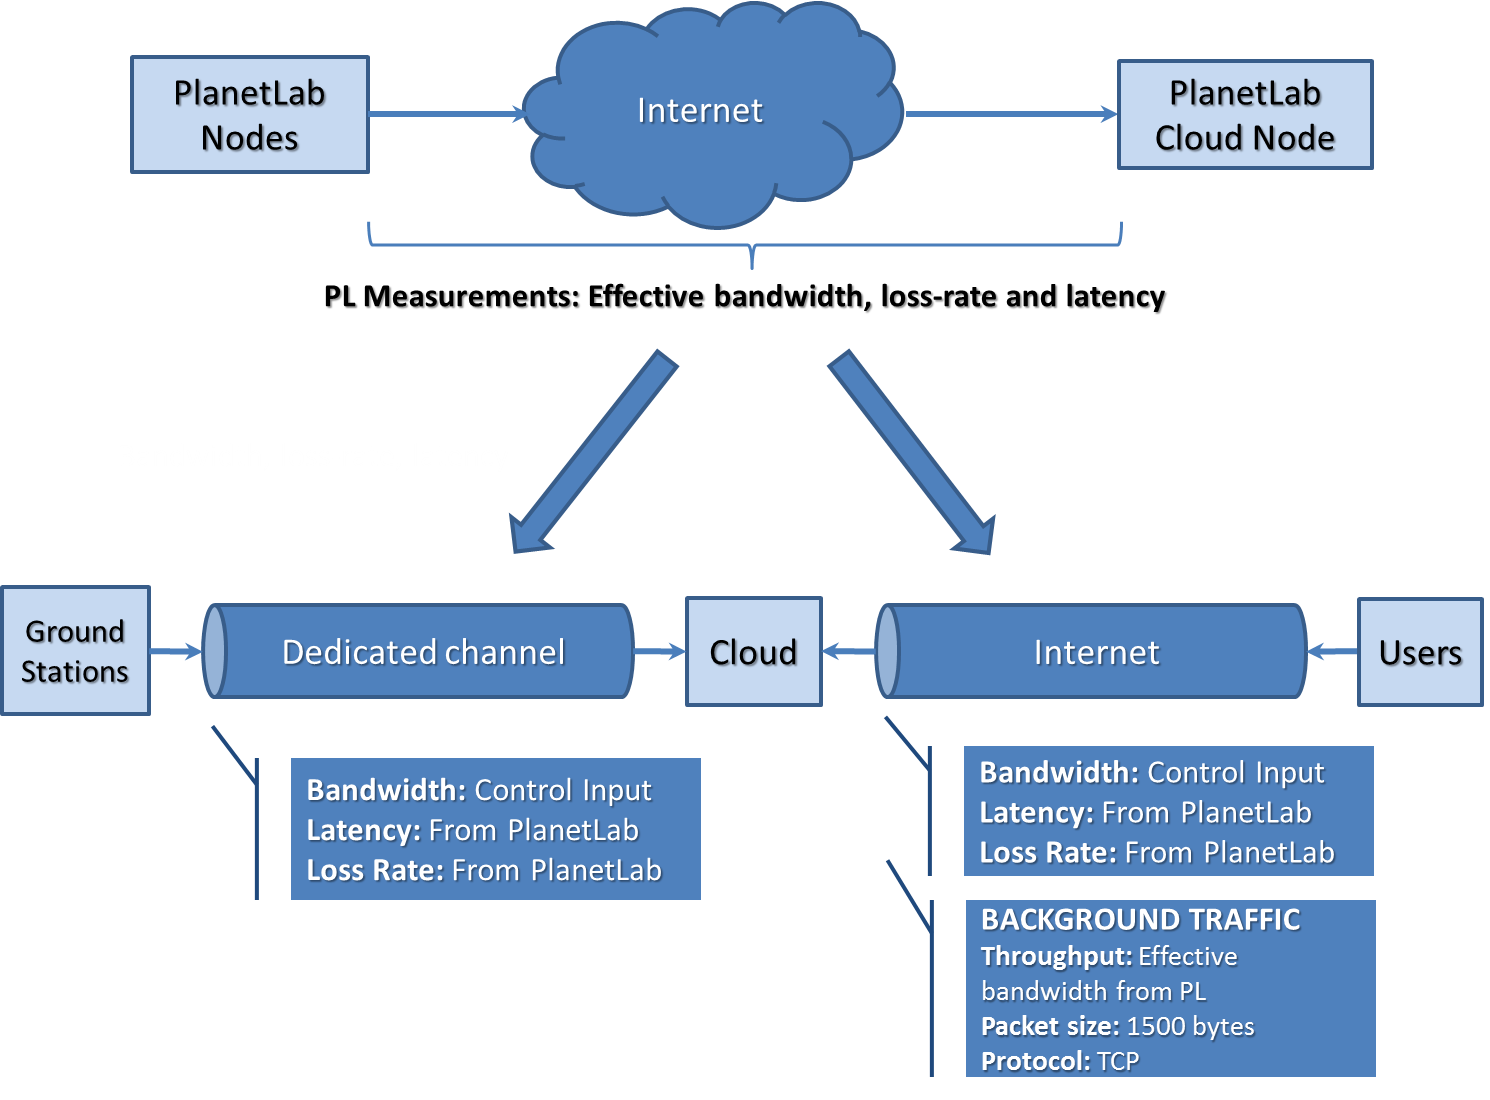
\includegraphics[width=5.22037in,height=3.85406in]{ple-img3.png} \par}

{\centering\bfseries
\label{bkm:Ref387240454}Figure\ 1. PlanetLab and Modelled Links
Equivalences.
\par}

\subsection[System modeling]{System modeling}
\hypertarget{Toc387315385}{}The real system is modeled into three main
components: i) a network of ground stations acquiring imagery data from
a constellation of optical satellites, ii) a cloud infrastructure that
ingests the data from the ground stations, processes it, stores it and
distributes it through web services and iii) end users around the world
accessing to the web services offered. The system can be divided into
two layers:\ 

\liststyleLFOv
\setcounter{saveenum}{\value{enumi}}
\begin{enumerate}
\setcounter{enumi}{\value{saveenum}}
\item Layer 1 is constituted by 12 ground stations connecting with a
cloud infrastructure.\ The ground stations and their location are
depicted in\ Table 1.\ Their locations and footprints are depicted in
Figure 2. The footprints represent the area in which the satellites can
establish the communication with the ground stations.
\end{enumerate}
{\centering\bfseries
\label{bkm:Ref387313886}Table\ 1\ Ground Stations Location
\par}

\begin{center}
\tablehead{}
\begin{supertabular}{|m{1.1295599in}|m{1.5712599in}|}
\hline
\bfseries Ground Station\  &
\bfseries Country of GS location\\\hline
\centering Irkutsk &
\centering\arraybslash Russia\\\hline
\centering Puertollano &
\centering\arraybslash Spain\\\hline
\centering Svalbard &
\centering\arraybslash Norway\\\hline
\centering Troll &
\centering\arraybslash Antarctic\\\hline
\centering Chetumal &
\centering\arraybslash Mexico\\\hline
\centering C\'ordoba &
\centering\arraybslash Argentina\\\hline
\centering Dubai &
\centering\arraybslash United Arab Emirates\\\hline
\centering Kourou &
\centering\arraybslash French Guiana\\\hline
\centering Krugersdorp &
\centering\arraybslash South Africa\\\hline
\centering Malaysia &
\centering\arraybslash Malaysia\\\hline
\centering Prince Albert &
\centering\arraybslash Canada\\\hline
\end{supertabular}
\end{center}

\bigskip

{\centering 
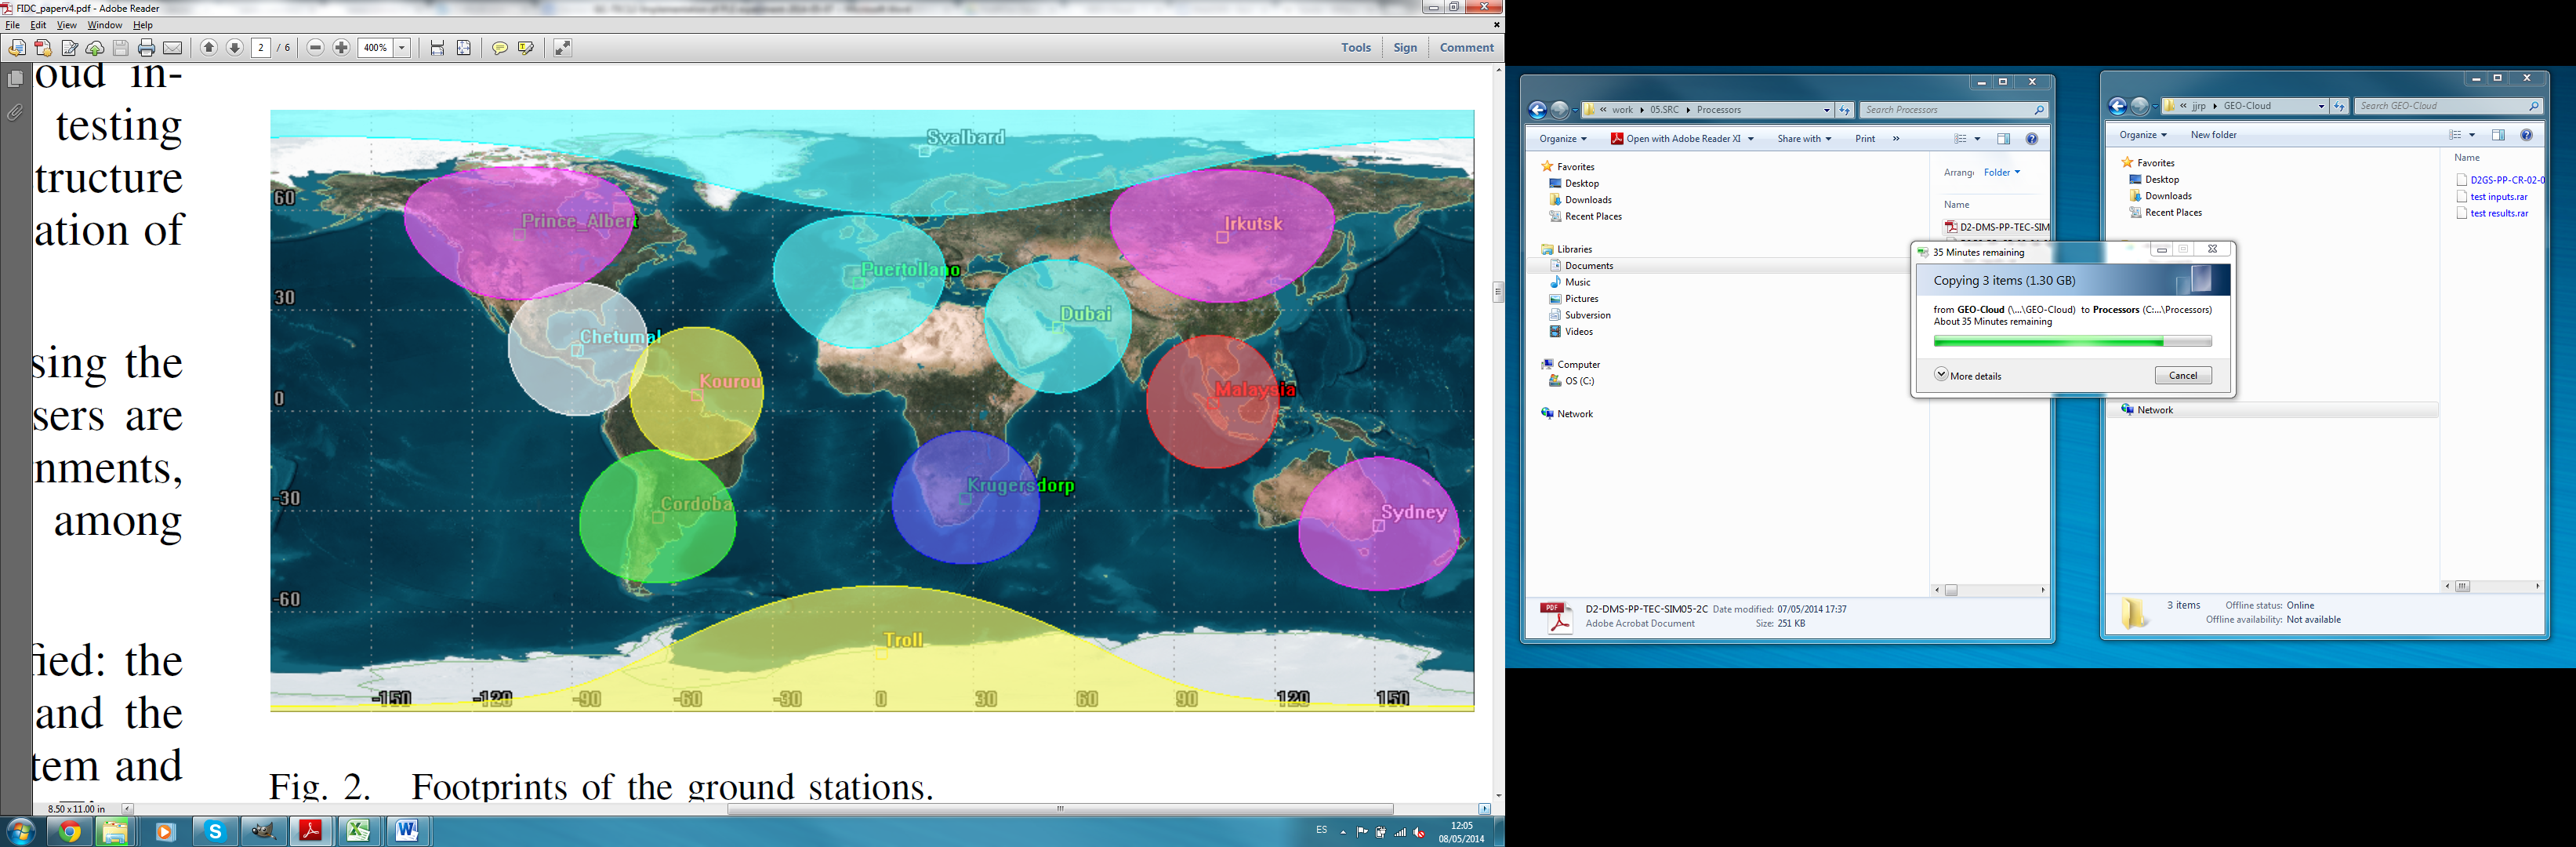
\includegraphics[width=5.37767in,height=2.68448in]{ple-img4.png} \par}

{\centering\bfseries
Figure\ 2\ Footprints of the ground stations.
\par}

\liststyleLFOv
\setcounter{saveenum}{\value{enumi}}
\begin{enumerate}
\setcounter{enumi}{\value{saveenum}}
\item Layer 2 is constituted by the end users accessing the\ web
services implemented in cloud. These users are\ distributed around the
world and can be governments,\ emergency services, media and
individuals among\ others.
\end{enumerate}
From the previous layers two networks can be identified: the network
between the ground stations and the cloud and the network between the
end users and the cloud. The system and the interconnections between
components\ are\ depicted in\ Figure 3. The connections between the
ground stations and end users with the cloud are represented as arrows
with different line types to represent that every connection can have
different characteristics and impairments.\ All the connections are
TCP.

{\centering 
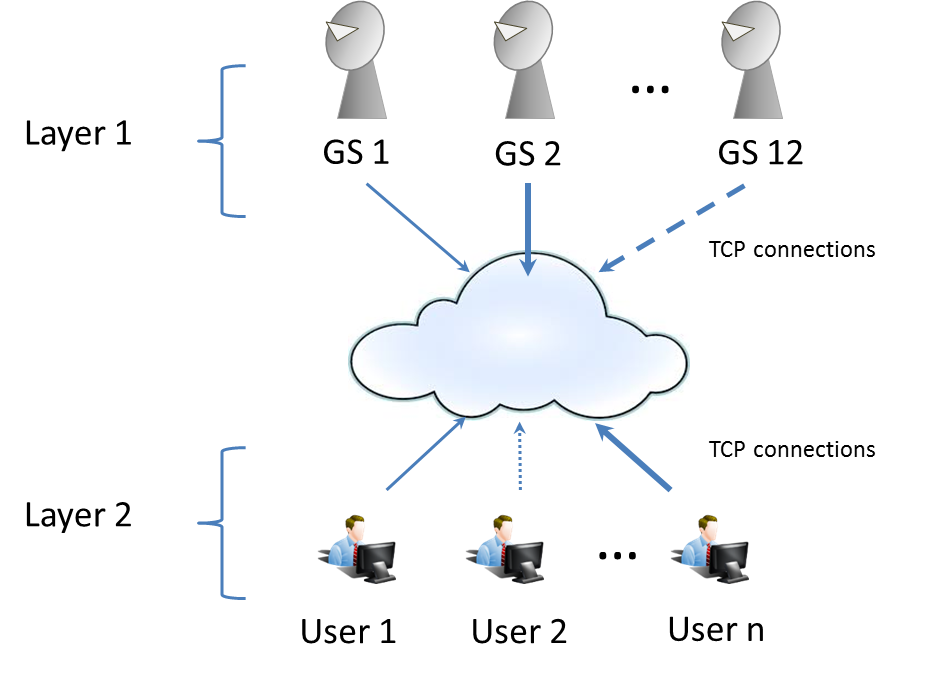
\includegraphics[width=3.35852in,height=2.41008in]{ple-img5.png} \par}

{\centering\bfseries
\label{bkm:Ref387314325}Figure\ 3\ System description
\par}


\bigskip

We define the network in function of the following representative
impairments:\ effective\ bandwidth, latency and loss rate. Thus, every
link is represented in function of the previous impairments:\ effective
bandwidth, latency, loss rate.

This system is implemented in Virtual Wall and BonFIRE as depicted
in\ Figure 4. The experiment in PlanetLab will be used to update the
network parameters connecting Virtual Wall and BonFIRE.

{\centering 
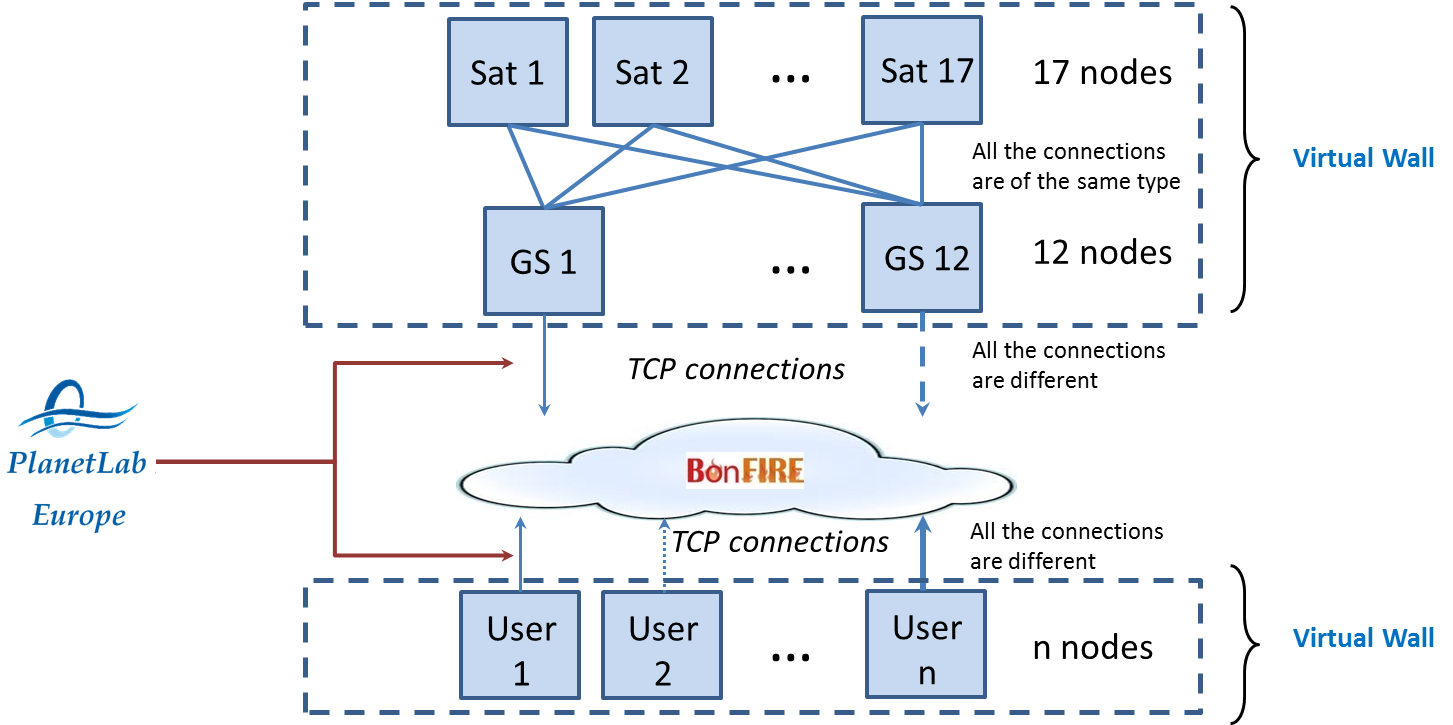
\includegraphics[width=5.48738in,height=2.73818in]{ple-img6.png} \par}

{\centering\bfseries
\label{bkm:Ref387318557}Figure\ 4\ Scheme of the system implemented in
GEO-Cloud
\par}


\bigskip

\subsection[Network Design\ in PlanetLab]{Network Design\ in PlanetLab}
\hypertarget{Toc387315386}{}
\bigskip

The model of the ground stations network, the cloud and the end users
accessing the web services provided was simplified to a set of
interconnected nodes. The network was divided into two layers connected
by a central node representing the cloud servers\ for similarity with
the real system:\ 

\liststyleLFOiv
\begin{itemize}
\item Layer 1: it represents the connections between 12 nodes
representing the ground stations and a central node representing the
cloud servers. In PlanetLab Europe and PlanetLab Central, the nearest
nodes to the real location of the ground stations were selected. For
the central node, a node in INRIA was chosen, since the BonFIRE cloud
has servers in the same location. This layer\ then\ represents the
transfer of geodata acquired by the constellation of satellites from
the ground stations in which the data is downloaded to the cloud.\ The
network topology implemented is peer-to-peer, i.e. each node
representing the ground stations is directly connected with the central
node. In\ Table 2\ the PlanetLab selected nodes for layer 1 and for the
cloud central node are shown. The nodes are numbered in ascending order
in function of the distance to the central node, i.e. the closest node
is the number 0 and the furthest the 37.\ 
\end{itemize}
{\centering\bfseries
\label{bkm:Ref387229383}Table\ 2. Ground Segement Nodes.
\par}

{\centering 
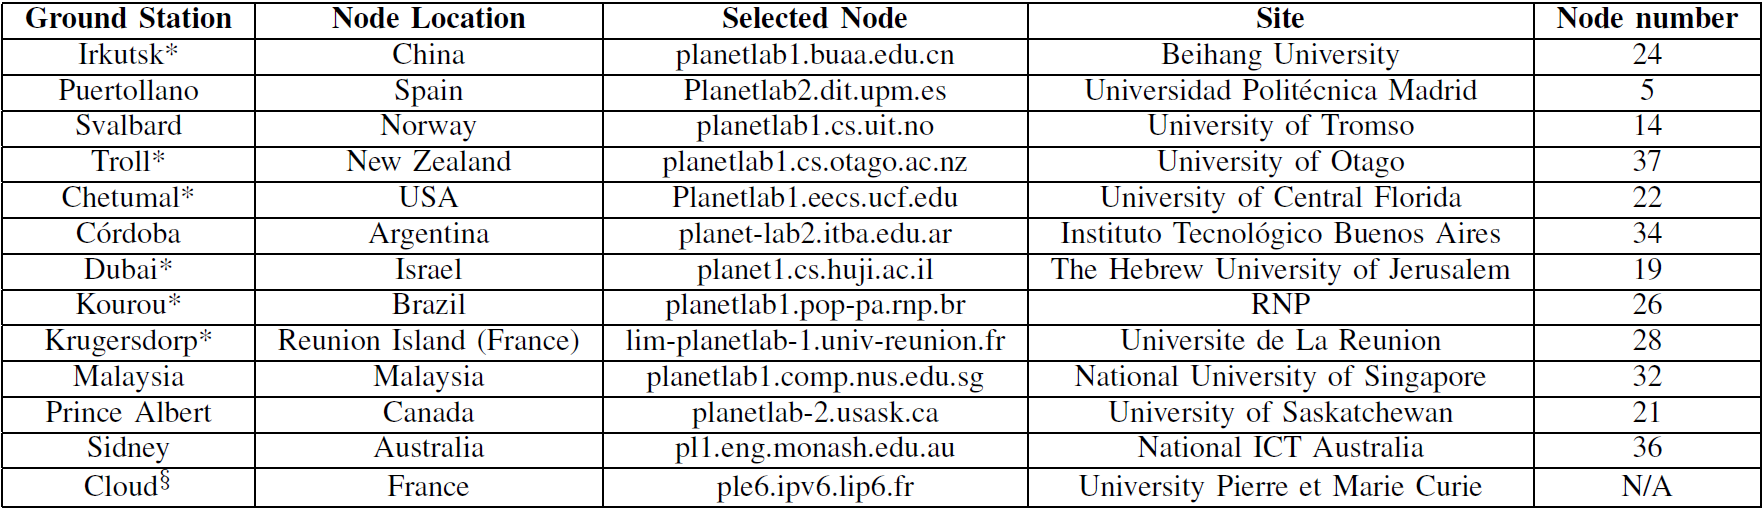
\includegraphics[width=6.20079in,height=1.79134in]{ple-img7.png} \par}

*\ These ground stations are located in\ areas without nodes, the
closest\ node has been selected.

{\S}\ Node representing the cloud infrastructure.

\liststyleLFOiv
\begin{itemize}
\item Layer 2: it represents the connection between the central node
representing the cloud servers and the end users. 31 different nodes
were selected in PlanetLab Europe and PlanetLab central in 31 different
countries around the world. This allows us to have a representative
sample of global users accessing the web services. In this case, the
network topology is also peer-to-peer. In\ Table 3\ the nodes selected
for layer 2 are listed. We tried to increase the number of nodes in
different countries, but during the execution of the experiment we did
not find available PlanetLab nodes in the following countries: Austria,
Cyprus, Denmark, Egypt,\ Ecuador, Iceland, India, Jordan, Mexico,
Pakistan, Puerto Rico, Romania, Slovenia, Sri Lanka, Tunisia, Turkey,
Venezuela, Uruguay and Taiwan.\ 
\end{itemize}
{\centering\bfseries
\label{bkm:Ref387229503}Table\ 3. Users Nodes.
\par}

{\centering 
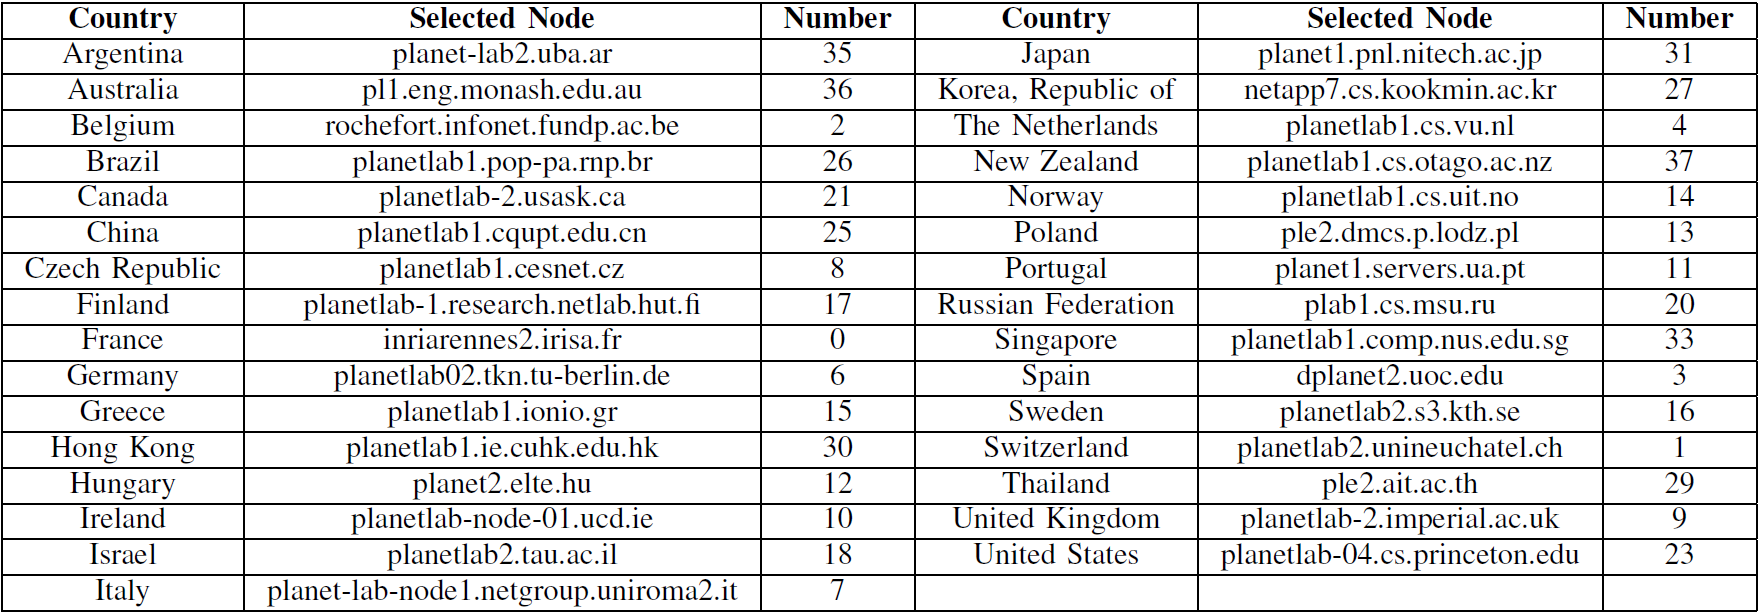
\includegraphics[width=6.1375in,height=2.1375in]{ple-img8.png} \par}

Figure 4\ shows a scheme representing the network created in
PlanetLab.\ The connections between the nodes are TCP.

{\centering 
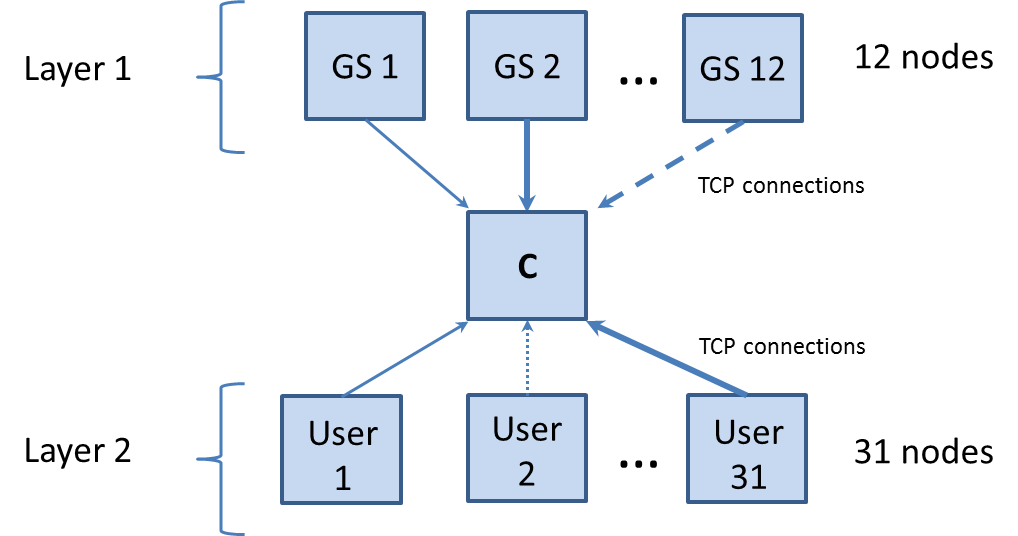
\includegraphics[width=4.01423in,height=2.11349in]{ple-img9.png} \par}

{\centering\bfseries
\label{bkm:Ref387229570}Figure\ 5. PlanetLab Network Scheme.
\par}

\subsection[Experiment Design\ and execution]{Experiment Design\ and
execution}
\hypertarget{Toc387315387}{}The experiment is designed to measure the
impairments of the network. Those impairments are required parameters
in Virtual Wall to deploy a topology network in such a testbed. Then,
in this experiment we measured latency, loss-rate
and\ effective\ bandwidth. The deployment of the experiment was done
with NEPI, in which Iperf and Ping were implemented to measure the
impairments. The experiment consists\ of establishing communications
between any node in layer 1 or layer 2 with the central node and
measuring the previously described impairments. 21600
trials\ will\ be\ done during 6 hours of the experiment execution in
steps of one second for each pair of nodes, i.e. a node from layer 1 or
2 and the central node.


\bigskip

The software developed to measure the impairments is constituted of 6
scripts:

\liststyleLFOvii
\setcounter{saveenum}{\value{enumi}}
\begin{enumerate}
\setcounter{enumi}{\value{saveenum}}
\item Script to measure the effective bandwidth in the ground stations
nodes: {\textquotedblleft}bandwidthGS.py{\textquotedblright}.\ 
\item Script to measure the effective bandwidth in the end users nodes:
{\textquotedblleft}bandwidthEndUser.py{\textquotedblright}
\item Script to measure the latency in the ground stations nodes:
{\textquotedblleft}latencyGS.py{\textquotedblright}.
\item Script to measure the latency \ in the end users nodes:
{\textquotedblleft}latencyEndUser.py{\textquotedblright}
\item Script to measure the loss rate in the ground stations nodes:
{\textquotedblleft}lossRateGS.py{\textquotedblright}
\item Script to measure the loss rate in the end users nodes:
{\textquotedblleft}lossRateEndUser.py{\textquotedblright}
\end{enumerate}
The pair of scripts that measure the same impairment are differentiated
one from each other in the provisioning of the nodes. Those nodes
representing the ground stations are manually selected, while the end
users nodes are automatically provisioned by NEPI by indicating the
country name as parameter.\ This parameter allows NEPI to select an
available node in that country.\ 


\bigskip

The previous six scripts are individually executed in a local host and
they start their workflow.


\bigskip

\subsubsection{The bandwidthGS.py script}
The bandwidthGS.py \ script measures the effective bandwidth in the
ground stations nodes.\ When it is executed it carries out the next
tasks:

\liststyleLFOviii
\setcounter{saveenum}{\value{enumi}}
\begin{enumerate}
\setcounter{enumi}{\value{saveenum}}
\item Provisioning of the nodes that were manually selected.
\item Creation of the commands to be uploaded:

\begin{itemize}
\item In the cloud node
\end{itemize}
\end{enumerate}
{\itshape
{\textgreater} timeout \%dm iperf -s -f m -i 1 -p \%d\ }

\textit{Timeout}\ is a command that executes a program during a
specified time\ \textit{\%dm}\ in minutes. For this
experiment\ \textit{dm}\ was chosen to be 65 minutes.

\textit{{}-s}\ indicates that Iperf is executed in server mode

\textit{{}-f m}\ indicates the format to report the received data. In
this case in Mb. \ 

\ \textit{{}-i}\textit{\ 1\ }Periodic reports every 1 second

\textit{{}-p}\textit{\ }\textit{\%d}\textit{\ }indicates the port to
listen. In our case 20004.


\bigskip

\liststyleLFOviii
\setcounter{saveenum}{\value{enumi}}
\begin{enumerate}
\setcounter{enumi}{\value{saveenum}}
\item \begin{itemize}
\item In the\ ground station\ nodes
\end{itemize}
\end{enumerate}
{\itshape
{\textgreater} iperf \ {}-i 1 -f m -c \%s\ {}-t \%d -p \%d \ {}-y c
{\textgreater} node\%d.out\ }

\textit{{}-i}\textit{\ 1\ }Periodic reports every 1 second.

\textit{{}-f m}\ indicates the format to report the received data. In
this case in Mb.

\textit{{}-c \%s\ }indicates the server to establish the communication
with.

\textit{{}-t\ }indicates the data transmission time. In our case 3600
seconds.

\textit{{}-}\textit{p}\textit{\ }\textit{\%d}\textit{\ }indicates the
port to listen. In our case 20004.

\textit{{}-y c}{\textgreater} node\%d.out\textit{\ }indicates\ that the
report format is csv. The output file is node\%d.out,
where\ \textit{\%d}\ indicates the number of the node tested.

By default Iperf is executed in TCP mode.

\liststyleLFOviii
\setcounter{saveenum}{\value{enumi}}
\begin{enumerate}
\setcounter{enumi}{\value{saveenum}}
\item Uploads\ the commands to the nodes
\item Executes the command in cloud
\item Executes the command in the rest of nodes
\item During the execution of the commands the data is collected
\item Finishes the execution of the commands\ 
\item The data collected is retrieved\ 
\item The resources are released.
\end{enumerate}
The flow diagram of the effective bandwidth measurements\ in the ground
station nodes\ is\ depicted in\ Figure 6\ a.


\bigskip

\subsubsection[The\ bandwidthEndUser.py script]{The\ bandwidthEndUser.py
script}
The\ bandwidthEndUser.py \ script measures the effective bandwidth in
the end users nodes. When it is executed it carries out the next tasks:

\liststyleLFOix
\setcounter{saveenum}{\value{enumi}}
\begin{enumerate}
\setcounter{enumi}{\value{saveenum}}
\item Automatic provisioning of the nodes.
\item Tasks 2 to 9 of the bandwidthGS.py script.
\end{enumerate}
The flow diagram of the effective bandwidth measurements\ in the end
users nodes\ is\ depicted in\ Figure 6\ b.

\subsubsection{The lossRateGS.py script}

\bigskip

The lossRateGS.py \ script measures the loss rate in the ground stations
nodes. When it is executed it carries out the next tasks:

\liststyleLFOx
\setcounter{saveenum}{\value{enumi}}
\begin{enumerate}
\setcounter{enumi}{\value{saveenum}}
\item Provisioning of the nodes that were manually selected.
\item Creation of the commands to be uploaded:

\begin{itemize}
\item In the cloud node
\end{itemize}
\end{enumerate}
{\itshape
{\textgreater} timeout \%dm iperf -s -f m -i 1 -p \%d -u}

\textit{Timeout}\ is a command that executes a program during a
specified time\ \textit{\%dm}\ in minutes. For this
experiment\ \textit{dm}\ was chosen to be 65 minutes.

\textit{{}-s}\ indicates that Iperf is executed in server mode

\textit{{}-f m}\ indicates the format to report the received data. In
this case in Mb. \ 

\ \textit{{}-i}\textit{\ 1\ }Periodic reports every 1 second

\textit{{}-p}\textit{\ }\textit{\%d}\textit{\ }indicates the port to
listen. In our case 20004.

\textit{{}-u}\ indicates that the Iperf software is executed in UDP
mode. \ 

\liststyleLFOviii
\setcounter{saveenum}{\value{enumi}}
\begin{enumerate}
\setcounter{enumi}{\value{saveenum}}
\item \begin{itemize}
\item In the ground station nodes
\end{itemize}
\end{enumerate}
{\textgreater}\ Iperf \ {}-i 1 -f m -c \%s -t \%d -p \%d\ {}-u\ {}-y c
{\textgreater} node\%d.out {\textquotedbl}

\textit{{}-i}\textit{\ 1\ }Periodic reports every 1 second

\textit{{}-f m}\ indicates the format to report the received data. In
this case in Mb.

\textit{{}-c \%s\ }indicates the server to establish the communication
with.

\textit{{}-t\ }indicates the data transmission time. In our case 3600
seconds.

\textit{{}-}\textit{p}\textit{\ }\textit{\%d}\textit{\ }indicates the
port to listen. In our case 20004.

\textit{{}-y c}{\textgreater} node\%d.out\textit{\ }indicates\ that the
report format is csv. The output file is node\%d.out,
where\ \textit{\%d}\ indicates the number of the node tested.

\textit{{}-u}\ indicates that the Iperf software is executed in UDP
mode. \ 


\bigskip

\liststyleLFOx
\setcounter{saveenum}{\value{enumi}}
\begin{enumerate}
\setcounter{enumi}{\value{saveenum}}
\item Uploads the commands to the nodes
\item Executes the command in cloud
\item Executes the command in the rest of nodes
\item During the execution of the commands the data is collected
\item Finishes the execution of the commands\ 
\item The data collected is retrieved\ 
\item The resources are released.
\end{enumerate}
The flow diagram of the\ loss rate\ measurements in the ground station
nodes\ is\ depicted in\ Figure 6\ a.

\subsubsection[The\ lossRateEndUser.py script]{The\ lossRateEndUser.py
script}
The\ lossRateEndUser.py \ script measures the\ loss rate\ in the end
users nodes. When it is executed it carries out the next tasks:

\liststyleLFOxi
\setcounter{saveenum}{\value{enumi}}
\begin{enumerate}
\setcounter{enumi}{\value{saveenum}}
\item Automatic provisioning of the nodes.
\item Tasks 2 to 9 of the\ lossRateGS.py script.
\end{enumerate}
The flow diagram of the loss rate measurements\ in the end users nodes
is\ depicted in\ Figure 6\ b.\ 

\subsubsection{The latencyGS.py script}
The latencyGS.py \ script measures the latency \ in the ground stations
nodes. When it is executed it carries out the next tasks:

\liststyleLFOxii
\setcounter{saveenum}{\value{enumi}}
\begin{enumerate}
\setcounter{enumi}{\value{saveenum}}
\item Provisioning of the nodes that were manually selected.
\item Creation of the commands to be uploaded:
\end{enumerate}
{\itshape
{\textgreater}ping \%s -w \%d}

\textit{\%s}\ indicates the host to do ping

\textit{{}-w}\textit{\ \%d}\ indicates the time of the ping
execution.\textit{\ }

\liststyleLFOxii
\setcounter{saveenum}{\value{enumi}}
\begin{enumerate}
\setcounter{enumi}{\value{saveenum}}
\item Uploads the commands to the nodes
\item Executes the command in cloud
\item Executes the command in the rest of nodes
\item During the execution of the commands the data is collected
\item Finishes the execution of the commands\ 
\item The data collected is retrieved\ 
\item The resources are released.
\end{enumerate}
The flow diagram of the\ latency\ measurements in the\ ground
station\ nodes\ is\ depicted in\ Figure 7\ a.

\subsubsection{The latencyEndUser.py script}

\bigskip

The latencyEndUser.py \ script measures the loss rate in the end users
nodes. When it is executed it carries out the next tasks:

\liststyleLFOxiii
\setcounter{saveenum}{\value{enumi}}
\begin{enumerate}
\setcounter{enumi}{\value{saveenum}}
\item Automatic provisioning of the nodes.
\item Tasks 2 to 9 of the latencyGS.py script.
\end{enumerate}

\bigskip

The flow diagram of the latency measurements in the end users nodes is
depicted in\ Figure 7\ b.

[Warning: Draw object ignored]

{\bfseries
\label{bkm:Ref387330064}Figure\ 6\ Workflow of the bandwidth and loss
rate measurement. (a) Workflow in the end users nodes. (b) Workflow in
the ground stations nodes.}


\bigskip

[Warning: Draw object ignored]

{\bfseries
\label{bkm:Ref387331646}Figure\ 7\ Workflow of the latency measurements.
(a) Workflow in the end users. (b) Workflow in the ground stations
nodes.\ }


\bigskip


\bigskip

\section[Conclusions]{Conclusions}
\hypertarget{Toc387315389}{}In this document the part of the GEO-Cloud
experiment executed in PlanetLab\ is presented. Topology networks have
been created in two layers to simulate the communications between the
ground stations and the cloud infrastructure and between such a cloud
infrastructure with end users around the world accessing web services
computed in cloud. The experiment consists of\ measuring the real
network impairments (effective\ bandwidth, latency and loss rate) to
obtain an approach for its later implementation in the complete Earth
Observation system simulator implemented in Virtual Wall and BonFIRE.\ 

\section[Bibliography]{Bibliography}
\hypertarget{Toc387315390}{}Europe, P. (2014). PlanetLab Europe
Project.\ \textit{PlanetLab Europe Project}. Retrieved from
http://www.planet-lab.eu/

INRIA. (2014). NEPI.\ \textit{NEPI}. Retrieved from
http://nepi.inria.fr/

Iperf. (2014). Iperf.\ \textit{Iperf}. Retrieved from http://iperf.fr/

Pelsser, C., Cittadini, L., Vissicchio, S., \& Bush, R. (2013). From
Paris to Tokyo: On the Suitability of ping to Measure
Latency.\ \textit{Proceedings of the 2013 conference on Internet
measurement conference}, (pp. 427-432). Retrieved from
http://conferences.sigcomm.org/imc/2013/papers/imc125s-pelsserA.pdf


\bigskip


\bigskip


\bigskip
\end{document}
